    %!TEX encoding = UTF-8 Unicode 
\documentclass[usenames,dvipsnames]{beamer}

    \usetheme{metropolis}

   \usecolortheme{seahorse}
   
        \usepackage{pgfpages}
\usepackage{CJKutf8} 
\usepackage{tcolorbox}
\usepackage[textfont={small}]{caption}

\usepackage{caption}
\captionsetup{skip=0pt,belowskip=-2mm}

    \setbeamercovered{invisible}
    \usepackage{tikz}   
    \usetikzlibrary{shapes,arrows}
\usepackage{graphicx}% http://ctan.org/pkg/graphicx
\usepackage{booktabs}
    \usepackage{framed, color}
    \definecolor{shadecolor}{rgb}{1, 0.8, 0.3}
    % To remove the navigation symbols from
    % the bottom of slides%
 %\setbeameroption{show notes on second screen}
%\setbeameroption{show only notes}
    \setbeamertemplate{navigation symbols}{}
    %
  \setbeamercolor{section in head/foot}{fg=black, bg=structure.fg!20!white}

\usepackage[natbibapa]{apacite}
\bibliographystyle{apacite}
\bibpunct{(}{)}{;}{a}{}{,}

\usetikzlibrary{calc}


\tikzstyle{decision} = [diamond, draw, fill=blue!20, 
    text width=4.5em, text badly centered, node distance=3cm, inner sep=0pt]
\tikzstyle{block} = [rectangle, draw, fill=blue!20, 
    text width=6em, text centered, rounded corners, minimum height=4em]
\tikzstyle{line} = [draw, -latex']
\tikzstyle{cloud} = [draw, ellipse,fill=red!20, node distance=3cm,
    minimum height=2em]

\newcommand{\tikzmark}[1]{\tikz[overlay,remember picture] \node (#1) {};}
\newcommand{\DrawBox}[1][]{%
    \tikz[overlay,remember picture]{
    \draw[red,#1]
      ($(left)+(-0.2em,0.9em)$) rectangle
      ($(right)+(0.2em,-0.3em)$);}
}

\newenvironment{variableblock}[3]{%
  \setbeamercolor{block body}{#2}
  \setbeamercolor{block title}{#3}
  \begin{block}{#1}}{\end{block}}

\makeatletter
\setbeamertemplate{footline}
{
  \leavevmode%
  \hbox{%
  \begin{beamercolorbox}[wd=1\paperwidth,ht=2.25ex,dp=1ex,center]{author in head/foot}%
    \usebeamerfont{author in head/foot}%
    \insertsectionnavigationhorizontal{0.8\paperwidth }{}{}%
     \insertframenumber /  \inserttotalframenumber
 \end{beamercolorbox}}%
 % \begin{beamercolorbox}[wd=.3\paperwidth,ht=2.25ex,dp=1ex,right]{date in head/foot}%
   % \usebeamerfont{date in head/foot}\insertshortdate{}\hspace*{2em}
  \hspace*{2ex} 
  %\end{beamercolorbox}}%
  \vskip0pt%
}


\usepackage{graphicx}
\usepackage[caption=false]{subfig}
\usepackage{multicol}
\usepackage{color, colortbl}
\definecolor{Gray}{gray}{0.9}

%\definecolor{white}{white}{0.9}

%\setbeamercovered{white}
    %\usepackage{bm} % For typesetting bold math (not \mathbold)
    %\logo{\includegraphics[height=0.6cm]{yourlogo.eps}}
\title{Are legislators more responsive to high quality evidence? A field experiment}
\author{Angèle Delevoye, Trevor Incerti and Sōm Duchébaggè}

\date{29 May 2019} 


\begin{document}
\maketitle

%%%%%%%%%%%%%%%%%%%%%%%%%%%%%%%%%%%

\section{Introduction}


\begin{frame}
\frametitle{Evidence-based policymaking: a bipartisan goal}

\begin{columns}
\column{0.5\textwidth}
\includegraphics[scale=0.35]{{"../figs/bill text"}.png} 

\column{0.3\textwidth}
\includegraphics[scale=0.35]{{"../figs/bill adoption"}.png} 


\end{columns}


\end{frame}

\begin{frame}
\frametitle{Research Questions}
\begin{itemize}
\item Do policymakers \textcolor{Cerulean}{give more credence} to high quality research?
\vspace{15mm}
\pause
\item Can policymakers \textcolor{Cerulean}{recognize} differences in research quality?
\end{itemize}
\end{frame}

%\item Heterogeneity by party \hyperlink{hte_party}{\beamerbutton{Figure}} and pre-existing nationalism \hyperlink{hte_nat}{\beamerbutton{Figure}} in Japan. 

%%%%%%%%%%%%%%%%%%%%%%%%%%%%%%%%%%%

\section{Theory}

\begin{frame}
\frametitle{Pre-existing literature}

\begin{itemize}
\item Literature on evidence use in policy-making, on relationship between science, researchers and policy-makers in a democracy 
\vspace{1cm}
\item Existing field/audit experiments reaching out to policy-makers \hyperlink{existing}{\beamerbutton{Figure}}
\end{itemize}

\end{frame}

%%%%%%%%%%%%%%%%%%%%%%%%%%%%%%%%%%%

\begin{frame}
\frametitle{Evidence standards}

\begin{itemize}
\item Evidence standards and descriptions already adopted in federal legislation.
\begin{itemize}
\item Secondary Education Act 65, No Child Left Behind 01, Every Student Succeeds Act 2015 (ESSA)
\end{itemize}
\pause
\vspace{0.5cm}
\item Department of Education (DoE) standards tiers under ESSA 2015:
\begin{itemize}
\item Strong causal evidence
\item Moderate causal evidence
\item Low causal evidence
\item High levels of specificity covering cluster-random assignment \hyperlink{doe_cluster}{\beamerbutton{Figure}}, IVs \hyperlink{doe_iv}{\beamerbutton{Figure}}, and missingness/attrition \hyperlink{doe_missing}{\beamerbutton{Figure}}, and RDs \hyperlink{doe_rd}{\beamerbutton{Figure}}. 
\end{itemize}
\pause
\item Other federal agencies have adopted similar standards \hyperlink{other_agencies}{\beamerbutton{Figure}}        
\end{itemize}

\end{frame}

%%%%%%%%%%%%%%%%%%%%%%%%%%%%%%%%%%%

\begin{frame}
\frametitle{Treatment 2, Information on evidence standards}
\scriptsize
\underline{From DoL's CLEAR database:}
\bigbreak
\textit{"\textcolor{Cerulean}{High Causal Evidence standards} mean there is strong evidence that the effects estimated in this study are solely attributable to the intervention being examined. This does not necessarily mean that the study found positive impacts, only that the analysis meets high methodological standards and the causal impacts estimated, whether positive, negative, or null, are credible. Currently, only \textcolor{Cerulean}{well-implemented randomized controlled trials} can receive this rating"}

\textit{"\textcolor{Cerulean}{Low Causal Evidence standards} mean there is little evidence that the effects estimated in the study are attributable to the intervention being examined, and other factors are likely to have contributed to the results. This does not imply that the study's results are not useful for some purposes, but they should be \textcolor{Cerulean}{interpreted with caution}. Causal studies that do not meet criteria for a high or moderate evidence rating receive this rating."}

\end{frame}


%%%%%%%%%%%%%%%%%%%%%%%%%%%%%%%%%%%

\section{Design}

\begin{frame}
\frametitle{Overview of experimental design}

\begin{itemize}
\item 2x2 factorial design with two treatments:
\begin{itemize}
\item Evidence standard (low vs. high)
\item Whether evidence standards are explained to policymakers
\end{itemize}
\end{itemize}

\vspace{5mm}
\begin{table}[H]
\centering
\caption{Treatment arms}
\label{tab: arms} 
\bigbreak
\begin{tabular}{|l|l|l|l|l|}
\hline
& \textbf{Lower Tier} & \textbf{Higher Tier} \\ \hline
\textbf{No information} & Control & High and no info \\ \hline
\textbf{Information} & Low and info & High and info \\ \hline
\end{tabular}
\end{table}

\end{frame}



%%%%%%%%%%%%%%%%%%%%%%%%%%%%%%%%%%%

\begin{frame}
\frametitle{Overview of DoE studies}

158 interventions examining 49 outcomes %with \textcolor{Cerulean}{366} unique combinations.

\textcolor{Cerulean}{12} interventions with significant results and same outcome, but analyzed by studies with two different research designs.

\vspace{-4mm}
\captionsetup{labelformat=empty}

\begin{table}[!htbp] \centering 
  \caption{} 
  \label{all_tiers} 
\tiny 
\begin{tabular}{@{\extracolsep{1mm}} ccc} 
\\[-1.8ex]\hline 
\hline \\[-1.8ex] 
 & Intervention & Outcome \\ 
\hline \\[-1.8ex] 
1 & ACT/SAT Test Preparation and Coaching Programs & General academic achievement (high school) \\ 
2 & Dual Enrollment Programs & Access and enrollment \\ 
3 & Dual Enrollment Programs & Attainment \\ 
4 & Knowledge is Power Program (KIPP) & English language arts achievement \\ 
5 & Knowledge is Power Program (KIPP) & General Mathematics Achievement \\ 
6 & Pre-K Mathematics & General Mathematics Achievement \\ 
7 & READ 180® & Comprehension \\ 
8 & READ 180® & Literacy achievement \\ 
9 & Success for All® & Alphabetics \\ 
10 & Success for All® & Comprehension \\ 
11 & Teach for America (TFA) & English language arts achievement \\ 
12 & Teach for America (TFA) & General Mathematics Achievement \\ 
\hline \\[-1.8ex] 
\end{tabular} 
\end{table} 


\end{frame}



%%%%%%%%%%%%%%%%%%%%%%%%%%%%%%%%%%%

\begin{frame}
\frametitle{Outcomes}

\begin{itemize}
\item Ideally: partner with a \textcolor{Cerulean}{3rd party organization} and examine: 
\begin{enumerate} 
\item Whether or not a \textcolor{Cerulean}{meeting was established}. 
\item Seniority of the individual with whom a successful meeting was granted (as in \citet{kalla2016campaign}).
\pause
\item [--] May also allow us to engage in participant observation (qualitative data)
\end{enumerate}
\pause
\vspace{1cm}
\item Alternatively: \textcolor{Cerulean}{email response rates}
\end{itemize}

\end{frame}






%%%%%%%%%%%%%%%%%%%%%%%%%%%%%%%%%%%

\begin{frame}
\frametitle{Treatment effect estimation}

Primary effects (ATE)
\begin{itemize}
\item Block random assignment.
\item $ATE = \sum_{j = 1}^{J} \frac{N_j}{N}ATE_j$
\begin{itemize}
\item Where $J$ is the number of blocks, blocks are indexed by $j$, and $\frac{N_j}{N}$ represents the share of subjects who belong to block $j$. 
\end{itemize}
\item P-values calculated using randomization inference.
\item Control group = Low quality evidence + no information
\vspace{0.5cm}
\end{itemize}
Heterogenous treatment effects (CATEs)
\begin{itemize}
\item Party, ..., ?
\item Note preregistration, multiple comparisons, and power.
\end{itemize}

\end{frame}

%%%%%%%%%%%%%%%%%%%%%%%%%%%%%%%%%%%

\begin{frame}
\frametitle{Power analysis assumptions}

\begin{itemize}
\item N = 535 (federal) and 1000 (state)
\vspace{0.5cm}
\item Low quality evidence + information provision = \textcolor{BrickRed}{-10\%}
\item High quality evidence + no information provision = \textcolor{Emerald}{+5\%}
\item High quality evidence + information provision = \textcolor{LimeGreen}{+12.5\%}
\vspace{0.5cm}
\item Standard deviation = 0.08
\end{itemize}

\end{frame}

%%%%%%%%%%%%%%%%%%%%%%%%%%%%%%%%%%%

\begin{frame}
\frametitle{Power analysis: federal}

\only<1>{
\begin{figure}
\vspace{-0.25cm}
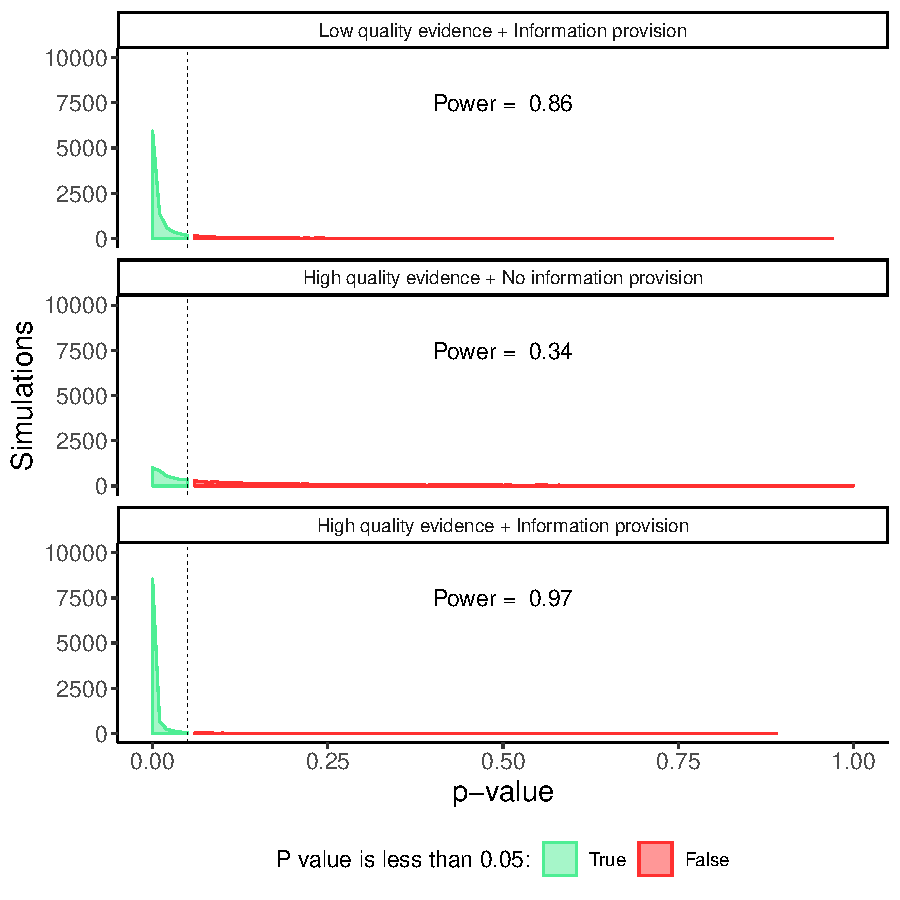
\includegraphics[scale=0.54]{../figs/power_fed.pdf}
\end{figure}
}

\end{frame}

%%%%%%%%%%%%%%%%%%%%%%%%%%%%%%%%%%%

\begin{frame}
\frametitle{Power analysis: state}

\only<1>{
\begin{figure}
\vspace{-0.25cm}
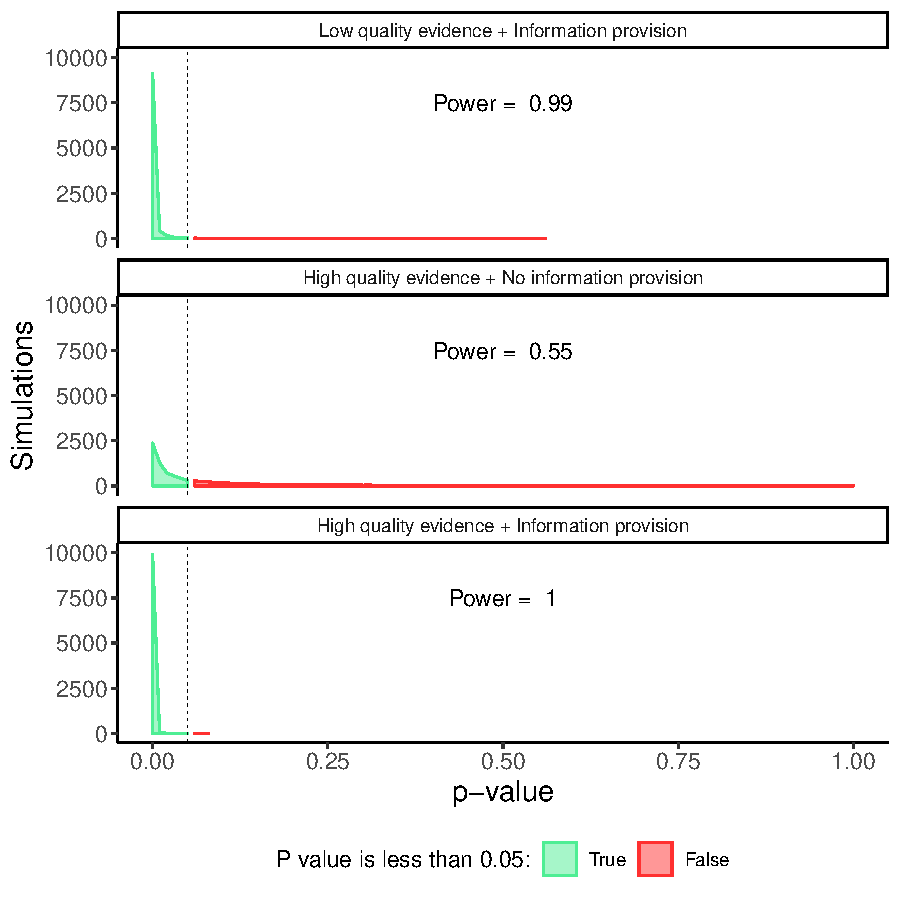
\includegraphics[scale=0.54]{../figs/power_state.pdf}
\end{figure}
}

\end{frame}

%%%%%%%%%%%%%%%%%%%%%%%%%%%%%%%%%%%



\section{Conclusion}

\begin{frame}
\frametitle{Timeline and questions}
\begin{itemize}
\item \textcolor{Cerulean}{Ideal timeline}: pre-registration and initial contact with 3rd party organization by end of 2019, roll-out of the experiment in the first half of 2020 (political context)
\item Use a \textcolor{Cerulean}{neutral or partisan policy} proposal?
\begin{itemize}
\item Partisan policy proposal might allow us to test legislator's motivated reasoning, but power issues.
\end{itemize}
\item Better \textcolor{Cerulean}{outcome measurements}?
\item Suggestions for kind of \textcolor{Cerulean}{organization to partner with}? Is organizational partnering feasible?
\item Federal, state, or local level?
\item Other suggestions?
\end{itemize}

\end{frame}


%%%%%%%%%%%%%%%%%%%%%%%%%%%%%%%%%%%
\appendix
%%%%%%%%%%%%%%%%%%%%%%%%%%%%%%%%%%%

\section{Supplemental material}



\begin{frame}[label= existing]
\frametitle{Existing field/audit experimens}




\begin{table}[]
\caption{Audit experiments conducted with U.S. policy-makers}
\label{tab:audit_experiments} 
\bigbreak
\tiny
\begin{tabular}{|l|l|l|l|l|l|l|l|l|}
\hline
Reference      
& Federal/State                                                                                                                        & Arms 
& Treatment                                                                                                           
& Design                                                                                                                                                        & Outcome 
& 3rd party?                                                                                                                                                                                                                                                  \\ \hline
 \citet{bergan2009does}        
& \begin{tabular}[c]{@{}l@{}}State \\ (New Hampshire) \end{tabular}                                                  & 1
& \begin{tabular}[c]{@{}l@{}} Contacted \\ by activists \end{tabular}                                           & \begin{tabular}[c]{@{}l@{}}Matched pairs \\ (multimembers districts)\\ Randomization within party\\ and district stratas\end{tabular}                         
& Roll Call votes                                                                                            
& \begin{tabular}[c]{@{}l@{}}Yes: coalition of \\ public health-related groups\\  organizing a grassroots email \\ lobbying campaign by activists\end{tabular}                                                                                              
  \\ \hline
 \citet{butler2011politicians}       & \begin{tabular}[c]{@{}l@{}}4,859 state legislators\\ (44 states)\end{tabular}                                                        & 2x3          & \begin{tabular}[c]{@{}l@{}}Black or \\ white name and\\ party (D/R/blank)\\ of email sender\end{tabular}            & \begin{tabular}[c]{@{}l@{}}Block randomization\\ by state, chamber, \\ party, and whether\\ legislator is up for \\ reelection\end{tabular}                   & \begin{tabular}[c]{@{}l@{}}Rate of response\\ to emails\end{tabular}                                       & No                                                                                                                                                                                                                                                          \\ \hline
 \citet{kalla2016campaign}     & \begin{tabular}[c]{@{}l@{}}US Congress \\ 191 offices that had \\ not yet sponsored bill \end{tabular} & 1            & \begin{tabular}[c]{@{}l@{}}Reveal in email that\\ prospective attendees had\\ contributed to campaigns\end{tabular} & \begin{tabular}[c]{@{}l@{}}Blocks of 3 offices: closest\\ similarity on multiple \\ covariates\\ 1 treated, 2 control in each\\ of the 64 blocks\end{tabular} & \begin{tabular}[c]{@{}l@{}}Rate of response\\ to emails and\\ seniority of proposed\\ meeting\end{tabular} & \begin{tabular}[c]{@{}l@{}}Yes: liberal political organization \\ trying to set meetings between offices\\ and constituents who had previously \\ given to campaigns. \\ Goal of the meetings: rally support for \\ a bill banning a chemical.\end{tabular} 
 \\ \hline
  \citet{doberstein2017whom}     & \begin{tabular}[c]{@{}l@{}}1,108 \\ Canadian bureaucrats\end{tabular} & 2x2           & \begin{tabular}[c]{@{}l@{}}Source of the\\ policy information \\(academic, think tanks, \\ research-based \\advocacy groups) \end{tabular} & \begin{tabular}[c]{@{}l@{}}Sources in \\treatment groups \\ were falsified \\  Pre treatment survey\\ for covariates \end{tabular} & \begin{tabular}[c]{@{}l@{}} Credibility assessment of \\each of 5 research articles \\ Based on summaries \\ And ranking of the 5 articles \end{tabular} & \begin{tabular}[c]{@{}l@{}}No.\end{tabular} 
   \\ \hline
  \citet{zelizer2018responsive}     & \begin{tabular}[c]{@{}l@{}}18 bills \\ 76 state legislators \end{tabular} & 1          & \begin{tabular}[c]{@{}l@{}}Assigned to in-person\\ briefings by a \\ committee staffer \end{tabular} & \begin{tabular}[c]{@{}l@{}}Treatment assigned \\ at legislator-bill \\ dyad level \\ block RA \end{tabular} & \begin{tabular}[c]{@{}l@{}} Cosponsorship of bills \\ Roll-call votes \end{tabular} & \begin{tabular}[c]{@{}l@{}}No.\end{tabular} 
     \\ \hline
  \citet{butler2011can}     & \begin{tabular}[c]{@{}l@{}}New Mexico State House \\ 70 legislators \end{tabular} & 1          & \begin{tabular}[c]{@{}l@{}}Received district-specific \\survey results on \\constituents' opinions \\on a bill \end{tabular} & \begin{tabular}[c]{@{}l@{}}35 matched pairs \end{tabular} & \begin{tabular}[c]{@{}l@{}} Cosponsorship of bills \\ Roll-call votes \end{tabular} & \begin{tabular}[c]{@{}l@{}}Use of University Logo \\ And email from \\ own researchers' address\end{tabular} 
       \\ \hline
  \citet{butler2012field}     & \begin{tabular}[c]{@{}l@{}}489 legislatives offices \\ 23 states \\ 1,036 letters \end{tabular} & 2x4        & \begin{tabular}[c]{@{}l@{}}Received letter \\ ethnicity of sender varied \\ 2 ethnicities \\  type of letter varied \\ 4 types (policy vs service, \\ level of knowledge) \end{tabular} & \begin{tabular}[c]{@{}l@{}}35 matched pairs \end{tabular} & \begin{tabular}[c]{@{}l@{}} Rate of response \\ Roll-call votes \end{tabular} & \begin{tabular}[c]{@{}l@{}}Yes: actual individuals \\ 200 students at BYU \\ Opened post office boxes \\ in their hometown \end{tabular} \\
\hline
\end{tabular}
\end{table}


\end{frame}

%%%%%%%%%%%%%%%%%%%%%%%%%%%%%%%%%%%

\begin{frame}[label= doe_evidence]
\frametitle{Evidence tiers}

\only<1>{
\begin{figure}
\vspace{-0.25cm}
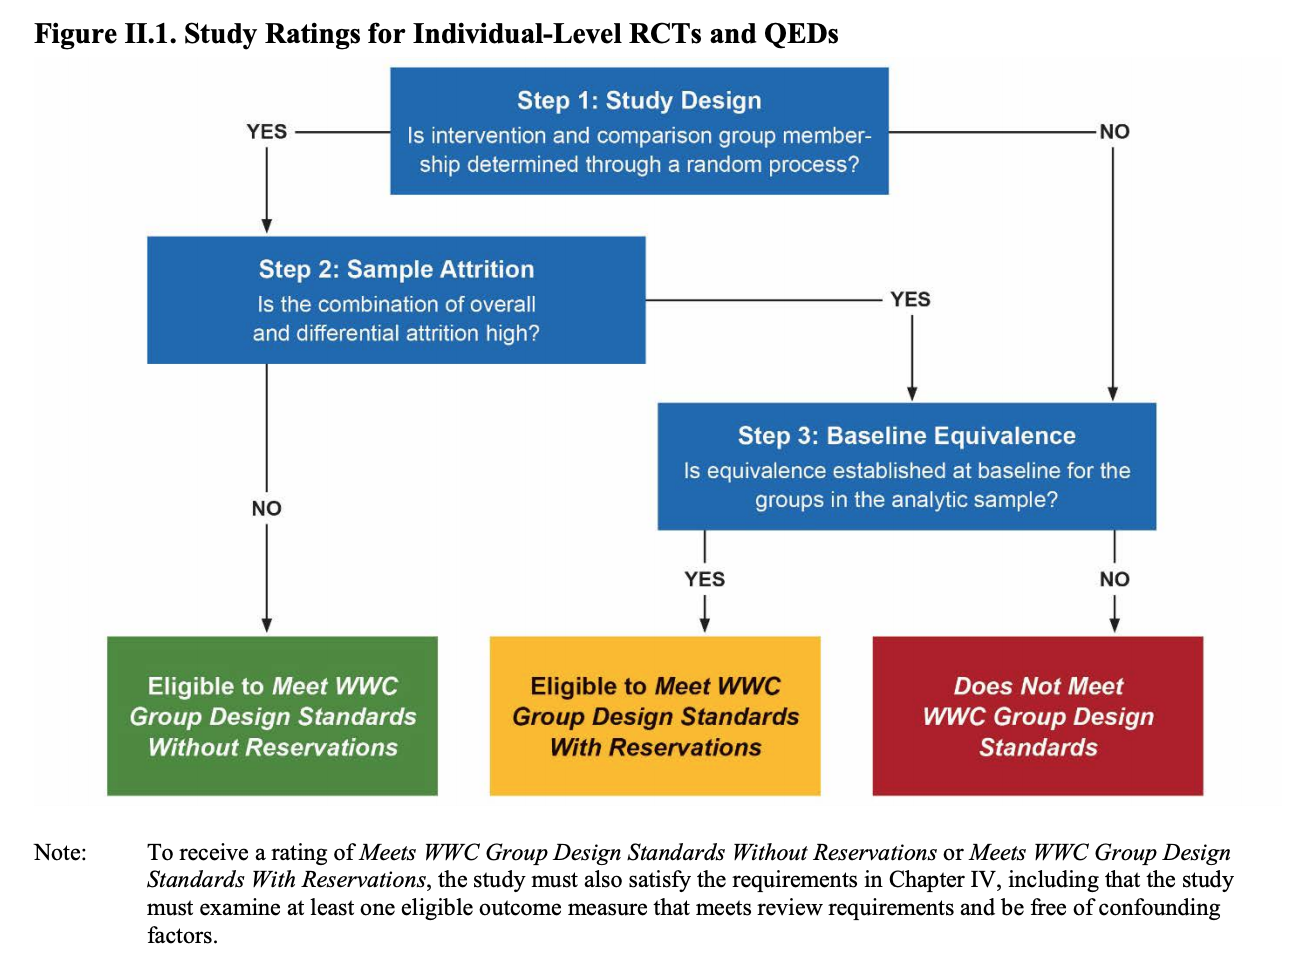
\includegraphics[scale=0.53]{../figs/DoE_standards.png} 
\end{figure}
}

\end{frame}

%%%%%%%%%%%%%%%%%%%%%%%%%%%%%%%%%%%

\begin{frame}[label= doe_cluster]
\frametitle{Evidence tiers: cluster random assignment}

\begin{center}
\vspace{-0.85cm}
\hspace*{-1cm}
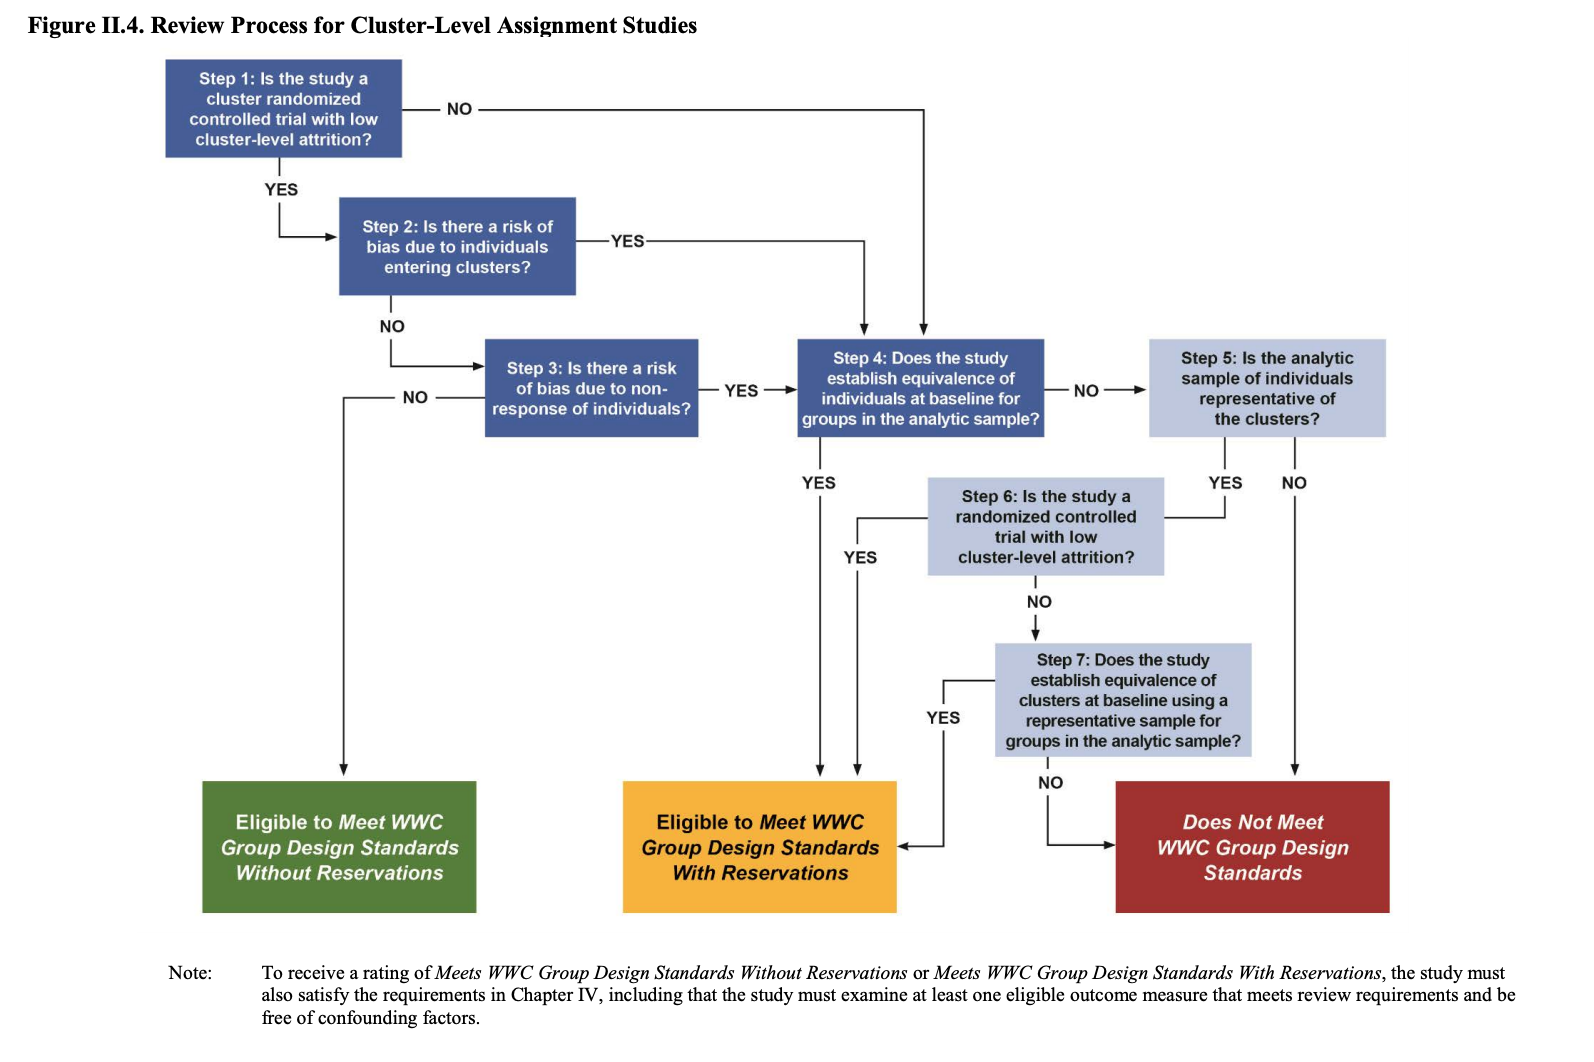
\includegraphics[scale=0.5]{../figs/DoE_clusters.png} 
\end{center}

\end{frame}

%%%%%%%%%%%%%%%%%%%%%%%%%%%%%%%%%%%

\begin{frame}[label= doe_iv]
\frametitle{Evidence tiers: instrumental variables}

\begin{center}
\vspace{-0.35cm}
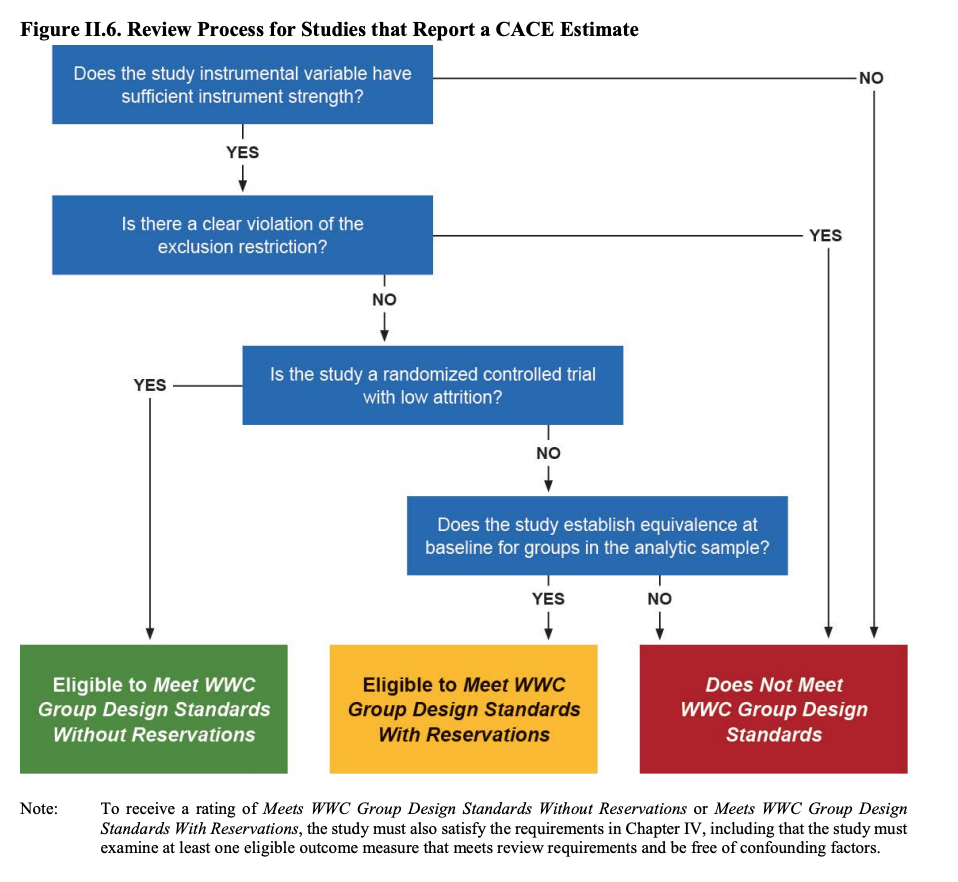
\includegraphics[scale=0.62]{../figs/DoE_CACE_IV.png} 
\end{center}

\end{frame}

%%%%%%%%%%%%%%%%%%%%%%%%%%%%%%%%%%%

\begin{frame}[label= doe_missing]
\frametitle{Evidence tiers: missingness and attrition}

\begin{center}
\vspace{-0.3cm}
\hspace*{-1cm}
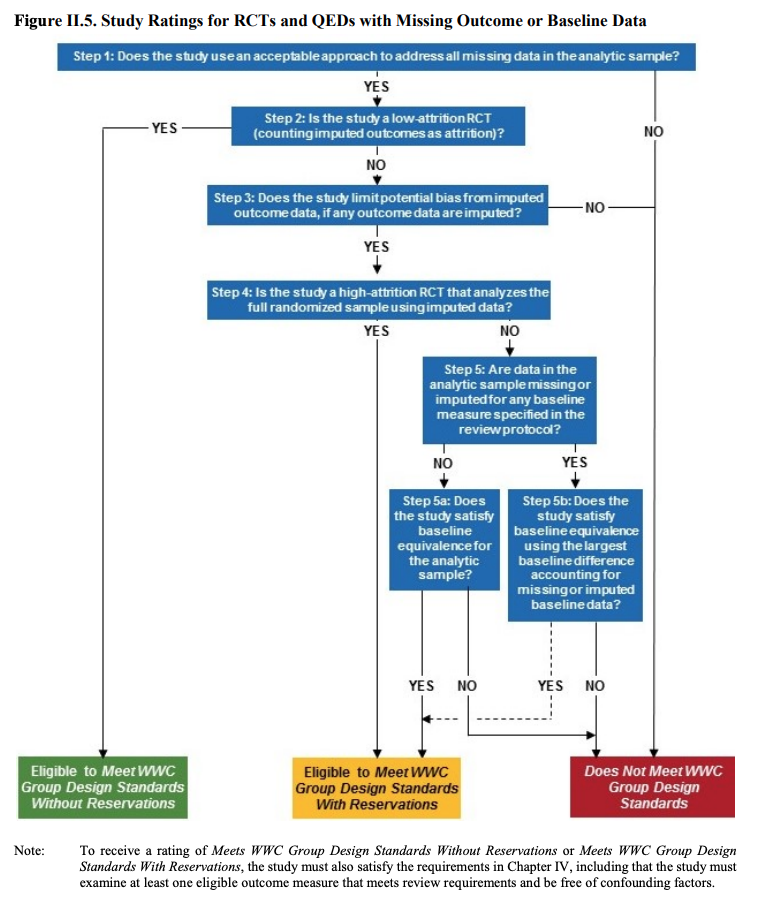
\includegraphics[scale=0.58]{../figs/DoE_missing.png} 
\end{center}

\end{frame}

%%%%%%%%%%%%%%%%%%%%%%%%%%%%%%%%%%%

\begin{frame}[label= doe_rd]
\frametitle{Evidence tiers: regression discontinuity}

\begin{center}
\vspace{-0.85cm}
\hspace*{-1cm}
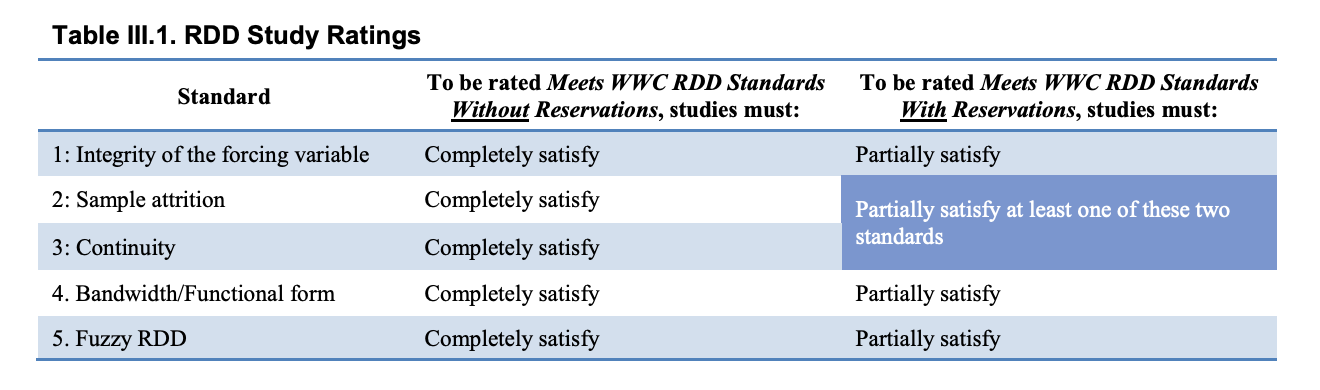
\includegraphics[scale=0.55]{../figs/DoE_RDs.png} 
\end{center}

\end{frame}

%%%%%%%%%%%%%%%%%%%%%%%%%%%%%%%%%%%

\begin{frame}[label= other_agencies]
\frametitle{Other federal evidence standards and databases}
\scriptsize
\begin{itemize}
	\item \textcolor{Cerulean}{Department of Labor} (DoL)'s CLEAR's clearinghouse: evidence on on labor topics 
	\item \textcolor{Cerulean}{Corporation for National and Community Service} (CNCS): evidence on what works in national service, social innovation, civic engagement, and volunteering
	\item \textcolor{Cerulean}{U.S. Agency for International Development} (USAID), YouthPower:  evidence on what works in youth and peacebuilding, youth and health, youth and agriculture, food security, and nutrition
	\item \textcolor{Cerulean}{US Departments of Agriculture and Defense}'s ClearingHouse for military family readiness: evidence on wide-ranging family and mental health issues. 
	\item \textcolor{Cerulean}{US Department of Health and Human services}: multiple databases on programs whose purpose is to prevent and/or reduce delinquency or other problem behaviors in young people, teen pregnancy and substance prevention programs, etc.
	\item \textcolor{Cerulean}{US Department of Justice}: multiple databases on drugs and substance abuse, juveniles, crime and crime prevention, victims and victimization, law enforcement, technology and forensics, corrections and reentry, and courts
\end{itemize}


\end{frame}






\bibliography{../doc/bibliography}
\end{document}